% PenCast showcase deck: one feature per slide, for recording a demo.
% Build: ./build.sh   (renders the videos/frames, then compiles with LuaLaTeX)
\documentclass[aspectratio=169,11pt]{beamer}
\usetheme[progressbar=frametitle,numbering=fraction]{metropolis}
% noplaybutton: media9's play-button layer hides a `cm` inside optional content, which Apple's PDF
% renderer skips, shifting everything after the video. PenCast's README explains.
\usepackage[noplaybutton]{media9}
\usepackage{animate}
\usepackage{amsmath}
\usepackage{fontawesome5}
\usepackage{tikz}
\usetikzlibrary{arrows.meta,positioning,calc}
\usepackage{pgfplots}
\pgfplotsset{compat=1.18}

% Colours from the app icon
\definecolor{pcIndigo}{HTML}{23246B}
\definecolor{pcViolet}{HTML}{7B4DFF}
\definecolor{pcSky}{HTML}{3D7BFF}
\setbeamercolor{frametitle}{bg=pcIndigo,fg=white}
\setbeamercolor{progress bar}{fg=pcViolet,bg=pcIndigo!25}
\setbeamercolor{title separator}{fg=pcViolet}
\setbeamercolor{alerted text}{fg=pcViolet}
\setbeamercolor{background canvas}{bg=white}
\setbeamercolor{palette primary}{bg=pcIndigo,fg=white}   % closing (standout) card

% \video{width}{name}{flashvars}: an MP4 from videos/ embedded in the PDF, poster shown until it plays.
\newcommand{\video}[3]{%
  \includemedia[width=#1,height=\dimexpr #1*9/16\relax,activate=pageopen,
    addresource=videos/#2.mp4,flashvars={source=videos/#2.mp4#3}]%
    {\includegraphics[width=#1]{videos/#2-poster}}{VPlayer.swf}}
\newcommand{\feature}[2]{\item[\textcolor{pcViolet}{#1}] #2}
\newcommand{\tryit}[1]{\par\vfill{\small\textcolor{pcViolet}{\faHandPointRight[regular]}\ \textit{#1}}}

\title{PenCast}
\subtitle{Beamer PDFs on iPad, with video, animation and ink}
\author{}
\date{}
\titlegraphic{\hfill
\includegraphics[height=1.5cm]{icon}}

\begin{document}

% ---------------------------------------------------------------- 1
\maketitle

% ---------------------------------------------------------------- 2
\begin{frame}{One PDF. No conversion.}
  \centering
  \begin{tikzpicture}[
      box/.style={draw=pcIndigo!35,fill=pcIndigo!4,rounded corners=6pt,minimum width=2.6cm,
                   minimum height=2.1cm,align=center,font=\small},
      arr/.style={-{Stealth[length=7pt]},very thick,pcViolet}]
    \node[box] (a) {{\Huge\textcolor{pcIndigo}{\faFile*[regular]}}\\[4pt]Write Beamer};
    \node[box,right=1.1cm of a] (b) {{\Huge\textcolor{pcIndigo}{\faCogs}}\\[4pt]Compile};
    \node[box,right=1.1cm of b] (c) {{\Huge\textcolor{pcIndigo}{\faPaperPlane[regular]}}\\[4pt]AirDrop};
    \node[box,right=1.1cm of c] (d) {{\Huge\textcolor{pcViolet}{\faTablet*}}\\[4pt]Present};
    \draw[arr] (a) -- (b); \draw[arr] (b) -- (c); \draw[arr] (c) -- (d);
  \end{tikzpicture}

  \vspace{1.2em}
  Videos, animations, links and overlays come \alert{straight from your PDF}:\\
  no PowerPoint step, no sidecar files, no special macros.
\end{frame}

% ---------------------------------------------------------------- 3
\begin{frame}{Embedded videos play in place}
  \begin{columns}[c]
    \begin{column}{0.6\textwidth}
      \video{\linewidth}{turing}{&autoPlay=true&loop=true}
    \end{column}
    \begin{column}{0.38\textwidth}
      \begin{itemize}
        \feature{\faFilm}{MP4s embedded with \texttt{media9} or a standard PDF Screen annotation}
        \feature{\faRedo}{Autoplay and loop settings come from the PDF}
        \feature{\faTv}{iPad and projector play the same video, in sync}
      \end{itemize}
    \end{column}
  \end{columns}
\end{frame}

% ---------------------------------------------------------------- 4
\begin{frame}{Write right over a playing video}
  \centering
  \video{0.64\textwidth}{waves}{&autoPlay=true&loop=true}
  \tryit{Circle the bright fringes where the two waves add up. Ink sits above the video on both screens.}
\end{frame}

% ---------------------------------------------------------------- 5
\begin{frame}{Tap a video to control it}
  \begin{columns}[c]
    \begin{column}{0.6\textwidth}
      \video{\linewidth}{vortex_pair}{}
    \end{column}
    \begin{column}{0.38\textwidth}
      \begin{itemize}
        \feature{\faPlay}{Tap: play / pause}
        \feature{\faSlidersH}{Drag to scrub through it}
        \feature{\faEyeSlash}{Controls stay on the iPad, never on the projector}
      \end{itemize}
      \vspace{0.5em}
      {\small An unequal counter-rotating vortex pair stirring two clouds of tracers.}
    \end{column}
  \end{columns}
\end{frame}

% ---------------------------------------------------------------- 6
\begin{frame}{\texttt{animate} sequences, frame-accurate}
  \centering
  \animategraphics[autoplay,loop,width=0.7\textwidth]{24}{frames/fourier-}{0}{47}

  \medskip
  A square wave from its first four harmonics, $\displaystyle\frac{4}{\pi}\sum_{k\,\mathrm{odd}}\frac{\sin kt}{k}$.
  \tryit{Frame rate and looping are read from the PDF. Tap the animation to pause it.}
\end{frame}

% ---------------------------------------------------------------- 7
\begin{frame}{Your notes survive every \texttt{\textbackslash pause}}
  \begin{columns}[t]
    \begin{column}{0.58\textwidth}
      \begin{align*}
        I &= \int_{-\infty}^{\infty} e^{-x^2}\,dx\\
        \uncover<2->{I^2 &= \iint_{\mathbb{R}^2} e^{-(x^2+y^2)}\,dx\,dy\\}
        \uncover<3->{&= \int_0^{2\pi}\!\!\int_0^{\infty} e^{-r^2}\,r\,dr\,d\theta\\}
        \uncover<4->{&= \pi \quad\Longrightarrow\quad \alert{I = \sqrt{\pi}}}
      \end{align*}
    \end{column}
    \begin{column}{0.38\textwidth}
      \vspace{1em}
      Annotate the first step:\\
      your ink \alert{stays} as each line appears.
      \tryit{Write on step one, then advance.}
    \end{column}
  \end{columns}
\end{frame}

% ---------------------------------------------------------------- 8
\begin{frame}{Point with the laser}
  \centering
  
\begin{tikzpicture}
    \begin{axis}[width=0.86\textwidth,height=0.58\textheight,axis lines=left,xlabel={$t$},
        ylabel={$x(t)$},xmin=0,xmax=20,ymin=-1.1,ymax=1.1,ticks=none,
        every axis plot/.append style={very thick}]
      \addplot[pcSky,samples=400,domain=0:20] {exp(-x/7)*cos(deg(2*x))};
      \addplot[pcViolet,dashed,samples=60,domain=0:20] {exp(-x/7)};
      \addplot[pcViolet,dashed,samples=60,domain=0:20] {-exp(-x/7)};
      \node[pcIndigo,font=\small] at (axis cs:15.5,0.62) {envelope $e^{-t/\tau}$};
      \node[pcIndigo,font=\small] at (axis cs:3.2,-0.95) {period $2\pi/\omega$};
    \end{axis}
  \end{tikzpicture}
  \tryit{Pick the laser: a glowing trail while you drag, gone when you lift. Or just a dot.}
\end{frame}

% ---------------------------------------------------------------- 9
\begin{frame}{Zoom in to write neatly}
  \begin{columns}[c]
    \begin{column}{0.56\textwidth}
      \centering
      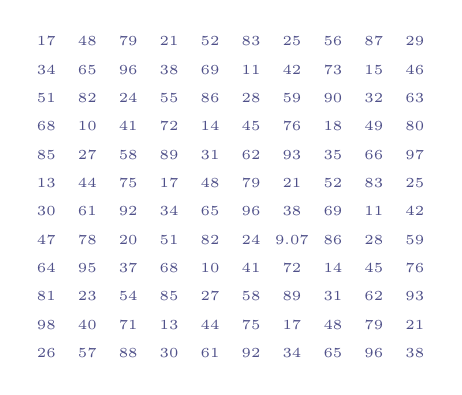
\begin{tikzpicture}[x=0.52cm,y=0.36cm]
        \foreach \r in {0,...,11} {
          \foreach \c in {0,...,9} {
            \pgfmathtruncatemacro{\v}{mod(17*\r + 31*\c + 7, 89) + 10}
            \ifnum\r=7 \ifnum\c=6 \def\v{9.07}\fi\fi
            \node[font=\tiny,text=pcIndigo!80] at (\c,-\r) {\v};
          }
        }
      \end{tikzpicture}
    \end{column}
    \begin{column}{0.42\textwidth}
      \begin{itemize}
        \feature{\faSearchPlus}{Pinch to zoom; one finger moves the page while you write}
        \feature{\faTv}{The projector can keep the whole slide, or follow your zoom}
        \feature{\faHandPaper[regular]}{Stray taps can't change slides while zoomed}
      \end{itemize}
      \tryit{One number in the table is not a whole number. Zoom in and circle it.}
    \end{column}
  \end{columns}
\end{frame}

% ---------------------------------------------------------------- 10
\begin{frame}{Lecture notes with a real fountain pen}
  \begin{columns}[t]
    \begin{column}{0.44\textwidth}
      \textbf{Example.} Find the eigenvalues of
      \[ A = \begin{pmatrix} 2 & 1\\ 1 & 2 \end{pmatrix}. \]
      \vspace{-0.5em}
      \begin{itemize}
        \feature{\faPenNib}{Round nib that follows Pencil pressure}
        \feature{\faSlidersH}{Tune how hard you press for thick and thin}
        \feature{\faDrawPolygon}{Lasso to move what you wrote}
      \end{itemize}
    \end{column}
    \begin{column}{0.54\textwidth}
      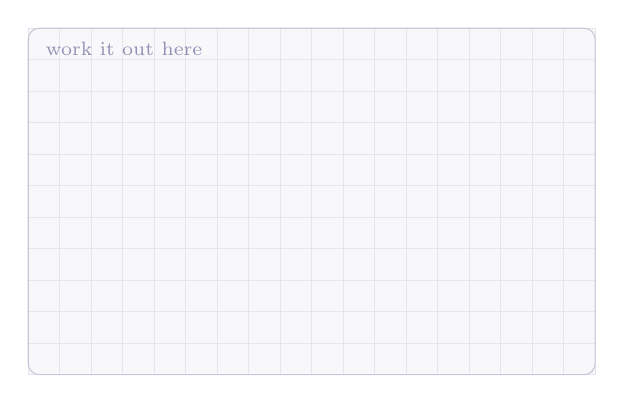
\begin{tikzpicture}[baseline=(current bounding box.north)]
        \fill[pcIndigo!3] (0,0) rectangle (7.2,4.4);
        \draw[pcIndigo!12,step=0.4] (0,0) grid (7.2,4.4);
        \draw[pcIndigo!25,rounded corners=4pt] (0,0) rectangle (7.2,4.4);
        \node[anchor=north west,font=\scriptsize,text=pcIndigo!50] at (0.1,4.35) {work it out here};
      \end{tikzpicture}
    \end{column}
  \end{columns}
\end{frame}

% ---------------------------------------------------------------- 11
\begin{frame}[label=links]{Links and navigation just work}
  \centering
  \vspace{1em}
  \scalebox{1.8}{\hyperlink{appendix}{\beamergotobutton{Jump to the appendix}}}

  \vspace{1.5em}
  Hyperref links, Beamer's navigation symbols, a Bluetooth clicker,\\
  arrow keys, swipes, or the slide grid: \alert{whatever you already use}.
\end{frame}

% ---------------------------------------------------------------- 12
\begin{frame}{Made for the room}
  \begin{columns}[t]
    \begin{column}{0.48\textwidth}
      \begin{itemize}
        \feature{\faTv}{Projector shows slide, video and ink; no toolbar}
        \feature{\faWifi}{HDMI or AirPlay; replug mid-talk without restarting}
        \feature{\faMoon[regular]}{Black, white or freeze the projector}
      \end{itemize}
    \end{column}
    \begin{column}{0.48\textwidth}
      \begin{itemize}
        \feature{\faStopwatch}{Talk timer}
        \feature{\faStickyNote[regular]}{Beamer speaker notes, on the iPad only}
        \feature{\faLaptop}{The same app on the Mac}
      \end{itemize}
    \end{column}
  \end{columns}
\end{frame}

% ---------------------------------------------------------------- 13
\begin{frame}{Take your notes with you}
  \centering
  \begin{tikzpicture}[
      card/.style={draw=pcIndigo!35,fill=white,rounded corners=4pt,minimum width=2.4cm,minimum height=1.35cm},
      lbl/.style={font=\small,align=center,text width=4.6cm}]
    \foreach \i in {0,1,2} \node[card] at (0.18*\i,-0.18*\i) {};
    \node[card,fill=pcViolet!8] at (0.36,-0.36) {\textcolor{pcViolet}{\faPenNib}};
    \node[lbl,below=0.25cm] at (0.2,-1.1) {\textbf{Notes}\\ one page per slide, final step, with your ink};
    \begin{scope}[xshift=6.5cm]
      \foreach \i in {0,...,5} \node[card] at (0.12*\i,-0.12*\i) {};
      \node[lbl,below=0.25cm] at (0.3,-1.1) {\textbf{Every page}\\ every overlay step, as presented};
    \end{scope}
  \end{tikzpicture}

  \vspace{0.8em}
  Tap \textbf{\faShareSquare[regular]} to save, share (AirDrop, Mail) or print, and send it to your students.
\end{frame}

% ---------------------------------------------------------------- 14
\begin{frame}[standout]
  
\includegraphics[height=2.2cm]{icon}\\[0.6em]
  PenCast\\[0.3em]
  {\normalsize Write Beamer. Present with ink.}
\end{frame}

\appendix
% ---------------------------------------------------------------- appendix
\begin{frame}[label=appendix]{Appendix: why $\int e^{-x^2}dx = \sqrt{\pi}$ needs polar coordinates}
  $e^{-x^2}$ has no elementary antiderivative, so the trick is to square the integral and
  switch to polar coordinates, where the extra factor $r$ makes $e^{-r^2}r$ integrable:
  \[ \int_0^\infty e^{-r^2} r\,dr = \tfrac12. \]

  \vspace{1em}
  \scalebox{1.6}{\hyperlink{links}{\beamerreturnbutton{Back}}}
\end{frame}

\end{document}
